\documentclass[11pt]{article}
\usepackage{tikz}
\usetikzlibrary{arrows.meta,positioning}
\usepackage{tabularx}
\usepackage{amsmath,amssymb,bm,graphicx,booktabs,hyperref,geometry}
\geometry{margin=1in}
\hypersetup{colorlinks=true, linkcolor=blue, citecolor=blue, urlcolor=blue}




\title{\textbf{Paper D-03: Geology:\\ A Constraint-Driven Flux Dynamics (CDFD) Perspective}}
\author{Steve Bico Mujjabi, MD\\
\small Independent Researcher\\
\small Founder, Vura Labs\\
\small Kampala, Uganda\\
\small ORCID: 0009-0001-0556-5516}
\date{May 2026}


\newcommand{\EarthSuppPath}{Part\_A\_Earth\_Systems/supplementary/supplementary\_earth\_}
\newcommand{\EngSuppPath}{Part\_B\_Engineered\_Systems/supplementary/supplementary\_eng\_}
\newcommand{\SocSuppPath}{Part\_C\_Socioeconomic\_Systems/supplementary/supplementary\_soc\_}
\newcommand{\DomainSuppPath}{Part\_D\_Domain\_Applications/supplementary/supplementary\_dom\_}
\begin{document}

\maketitle
\newpage


\begin{abstract}
In this paper we apply Adaptive Flux Limitation (AFL) to geology and geophysics, modelling
tectonic and volcanic processes as constrained transport systems. The potential $\Phi = \Phi_{tect}
+ \Phi_{magma} + \Phi_{fluid}$ encodes plate motion, magmatic, and hydrothermal fluxes; constraint
$C = C_{friction} + C_{crustal} + C_{viscosity}$ encodes fault friction, crustal rigidity, and
magmatic viscosity. The Surface Operating Ratio $\Psi_s^* = J/C$ classifies geological states from
stable inter-seismic loading through earthquake rupture and volcanic eruption.

We model the hypothesis that Gutenberg-Richter scaling, the seismic cycle, eruption styles, plate
velocity-size scaling, and Venus/Earth comparisons all emerge from AFL flux--constraint dynamics.

\textbf{Status: Inferred from AFL first principles; quantitative predictions are hypothesis-level.}\\
\textbf{Series tag: Dom-D03}
\end{abstract}

\section*{Symbol Conventions}

\noindent\textbf{CDFD/AFL Part IV symbol convention.}
\begin{center}
{\small
\begin{tabular}{p{0.15\linewidth}p{0.34\linewidth}p{0.41\linewidth}}
\hline
Symbol & Part IV meaning & Cross-domain reading \\
\hline
$\Phi$ & Driving flux or throughput & Energy, matter, signal, capital, information, traffic, force, or biological load entering a system \\
$C$ & Active constraint or capacity burden & Bottleneck, resistance, boundary, scarcity, toxicity, regulation, topology, latency, or load-bearing limit \\
$S$ & Responsiveness or adaptive surface & The system's ability to reconfigure, buffer, route, repair, learn, or preserve function under changing load \\
$M_s$ & Structural memory & Stored damage, hysteresis, inherited topology, institutional memory, trained weights, ecological legacy, or retained state \\
$\Psi_s$ & Adaptive operating ratio $(\Phi/C)\cdot S\cdot M_s$ & Local bookkeeping gauge for constrained operation, overload, recovery, or regime change; not a universal constant \\
$\Lambda$ & Life Number or capstone surplus ratio where explicitly defined & Reserved for Part II-derived life-number notation or synthesis-level surplus measures, never an undefined decoration \\
\hline
\end{tabular}
}
\end{center}

\noindent\textbf{Greek-symbol convention.}
\begin{center}
{\small
\begin{tabular}{p{0.15\linewidth}p{0.34\linewidth}p{0.41\linewidth}}
\hline
Symbol & Local role & Interpretation rule \\
\hline
$\alpha$ & Accumulation or reinforcement coefficient & Sets how fast a pathway, constraint, habit, cascade, or retained structure grows under load \\
$\beta$ & Relaxation, decay, clearance, or washout coefficient & Sets loss, recovery, damping, forgetting, degradation, or return toward baseline \\
$\gamma$ & Coupling, diffusion, redistribution, or transfer coefficient & Sets spread across nodes, layers, tissues, markets, infrastructures, media, or physical phases \\
$\delta,\epsilon$ & Perturbation, tolerance, small offset, or numerical guard & Used only as local thresholds, stability margins, measurement tolerances, or stress increments \\
$\eta,\lambda,\mu,\nu$ & Efficiency, rate, baseline, intensity, or frequency terms & Meaning is fixed by the equation, subscript, and domain-specific proxy in the paragraph where the term appears \\
$\rho,\sigma,\tau,\phi$ & Density/correlation, variability/noise, time-scale, phase, or field terms & Local coefficients only; subscripts bind them to the named pathway, domain, or experiment \\
$\Omega,\Lambda$ & Domain/state space; Life Number where defined & $\Omega$ names a modeled state space; $\Lambda$ carries life-number or synthesis notation only when the paper defines it \\
\hline
\end{tabular}
}
\end{center}


\section{Series Context}

Part I sets the flow--constraint language used here \cite{MujjabiPartI2026}. Part II develops the Life Number and the origins-of-life use of the same notation \cite{MujjabiPartII2026}. Part III applies AFL to biology and medicine \cite{MujjabiPartIII2026}. Part IV \cite{MujjabiPartIV2026}, DOI \url{https://doi.org/10.5281/zenodo.20395901}, is the cross-domain stress test: it asks where the notation clarifies measurement, and where it becomes only a metaphor.

\section{Introduction}


\subsection{The Mujjabi Universal Capacity Law}
Building directly upon the Fundamental Physics (Part I) \cite{MujjabiPartI2026}, the \textbf{Mujjabi Universal Capacity Law} proposes that across all scales---from black hole event horizons to global financial markets and power grids---driving high flux ($\Phi$) against a rigid topological constraint ($C$) can drive system saturation. When $\Phi/C$ approaches critical thresholds, the system does not scale linearly; it undergoes a topological phase transition.

\subsection{The Mujjabi Universal Memory Law}
The \textbf{Mujjabi Universal Memory Law} frames persistent systemic collapse. When a complex network fails to clear its structural memory ($M_s$) and its relaxation parameter decays ($\tau_{relax} \to \infty$), temporary stressors become permanent rigidities. This is the proposed CDFD mechanism behind ecological death, economic depressions, and infrastructural gridlock.


Earth's lithosphere moves at 1--10 cm/year, accumulating $\sim10^{18}$ J/year of seismic energy
at fault boundaries. This energy is released episodically in earthquakes, ranging from magnitude
1 (microseismic) to magnitude 9.5 (1960 Valdivia event, which released $\sim10^{23}$ J). The
Gutenberg-Richter law --- the power-law frequency-magnitude relationship observed in every seismic
catalogue worldwide --- is one of geology's most robust empirical observations, yet its mechanistic
origin has remained debated.

Volcanic systems provide a parallel AFL process: magma generated by partial melting of the mantle
must overcome crustal constraint to erupt. The 1991 Pinatubo eruption injected $\sim$10 km$^3$
of material and temporarily cooled global average temperature by 0.5$^\circ$C --- an AFL constraint
failure of planetary significance.

AFL provides a unified framework for both seismic and volcanic systems: both are instances of
potential accumulation against constraint, with episodic failure when $\Psi_s^* > 1$. The AFL
geological framework connects to the Part~IV Earth series: volcanic outgassing drives atmospheric
$\Phi$ (Paper~02); tectonic cycling controls long-term carbon sequestration and climate (Paper~10);
earthquake cascades resemble the systemic crisis propagation model of Paper~33.

\section{Core Hypothesis}

\begin{center}
\textit{
Geological systems are AFL flux--constraint systems in which tectonic and magmatic potential
$\Phi$ accumulates against crustal, frictional, and viscous constraint $C$: earthquakes are AFL
phase transitions when $\Psi_{s,seismic} > 1$ and fault friction is overcome; volcanoes erupt when
$\Psi_{s,magma} > 1$ and crustal strength is exceeded; the Gutenberg-Richter law emerges from AFL
constraint heterogeneity across the crust.
}
\end{center}

AFL geological hypothesis: the seismic cycle --- inter-seismic loading, critical state, rupture,
post-seismic relaxation --- is an AFL limit cycle:
\begin{equation}
\frac{d\sigma}{dt} = \dot{\sigma}_{loading} - \gamma_{rupture} \sigma \cdot \mathbb{1}[\sigma > \sigma_{cr}],
\end{equation}
where $\sigma$ is fault stress ($\Phi$), $\dot{\sigma}_{loading}$ is the tectonic loading rate
($S$), and $\gamma_{rupture}$ is the rupture propagation rate. The Gutenberg-Richter exponent
$b \approx 1$ emerges from AFL constraint heterogeneity: if $C_{friction}$ is exponentially
distributed across the fault system, then earthquake magnitudes (proportional to $\log(A_{rupture})$)
follow a power law.
\textbf{Status: Hypothesis; Gutenberg-Richter derivation requires AFL heterogeneity analysis.}

\section{Geological Potential Fields}

We define the generalised geological potential:
\begin{equation}
\Phi = \Phi_{tect} + \Phi_{magma} + \Phi_{fluid}
\end{equation}
where:
\begin{itemize}
    \item $\Phi_{tect}$ --- tectonic stress potential (accumulated elastic strain energy at fault
          systems; primary driver of seismicity; scales with plate convergence/divergence rate and
          fault locking degree);
    \item $\Phi_{magma}$ --- magmatic pressure potential (melt fraction $\times$ density contrast;
          drives volcanic systems; accumulates in magma reservoirs over decades to centuries;
          released explosively or effusively when crustal constraint is overcome);
    \item $\Phi_{fluid}$ --- hydrothermal fluid potential (pore pressure in fault zones; reduces
          effective normal stress; key trigger for induced seismicity from wastewater injection).
\end{itemize}

\section{Geological Constraint Axes}

\begin{equation}
C = C_{friction} + C_{crustal} + C_{viscosity}
\end{equation}

\begin{table}[h]
\centering
\caption{Geological constraint axes and AFL mechanisms.}
\begin{tabularx}{\textwidth}{@{}lXX@{}}
\toprule
Constraint axis & Geological substrate & AFL role \\
\midrule
$C_{friction}$ & Fault zone friction (Byerlee's law) & Primary seismic constraint; overcomes at rupture \\
$C_{crustal}$ & Crustal rigidity and yield strength & Volcanic pathway constraint; fails at eruption \\
$C_{viscosity}$ & Magma viscosity (silica, temperature) & Eruption style control; high viscosity = explosive \\
$C_{pore}$ & Fluid pore pressure & Reduces effective friction; induced seismicity driver \\
$C_{overburden}$ & Lithostatic pressure & Depth-dependent constraint on all geological fluxes \\
\bottomrule
\end{tabularx}
\end{table}

\subsection{Adaptive Surface Dynamics: Memory and Responsiveness}

The operating ratio $\Psi_s^*$ is mediated by adaptive surface components:
\begin{equation}
\Psi_s^* = (\Phi/C) \cdot S \cdot M_s
\end{equation}
where $S$ (Surface Responsiveness) and $M_s$ (Surface Memory) evolve as:
\begin{align}
\frac{dS}{dt} &= \kappa_s (\Psi_s^* - S) \\
\frac{dM_s}{dt} &= \Phi S - d_m M_s
\end{align}
These components represent the homeostatic capacity of the system to regulate its own operating ratio through memory and responsiveness.

\section{Flux Law}

Tectonic and volcanic throughput:
\begin{equation}
J_{geological} = -\frac{1}{C}\nabla \Phi
\end{equation}
where:
\begin{itemize}
    \item For seismic systems: $J_{seismic} = $ fault slip rate; $\nabla\Phi = $ stress gradient
          along fault; $C = C_{friction}$ (Byerlee friction coefficient $\times$ normal stress);
    \item For volcanic systems: $J_{volcanic} = $ magma ascent rate (m/s); $\nabla\Phi = $ magma
          pressure gradient (overpressure relative to lithostatic); $C = C_{viscosity} + C_{crustal}$;
    \item For hydrothermal systems: $J_{fluid} = $ fluid flux (Darcy's law); $\nabla\Phi = $ pore
          pressure gradient; $C = $ permeability$^{-1}$ (inverse permeability).
\end{itemize}

\section{Conservation Dynamics}

Geological potential evolves as:
\begin{equation}
\frac{\partial \Phi}{\partial t} = \nabla \cdot \left(\frac{1}{C}\nabla \Phi\right) + S
\end{equation}
where $S$ represents:
\begin{itemize}
    \item \textbf{Tectonic loading}: $S_{tect} = \dot{\sigma}_{plate}$ (far-field plate velocity
          $\times$ elastic modulus / fault locked length; steady background loading);
    \item \textbf{Magma generation}: $S_{magma}$ from mantle partial melting (proportional to
          mantle temperature anomaly and volatile content);
    \item \textbf{Glacial unloading}: $S_{glacio} > 0$ as ice sheets melt (reduces $C_{overburden}$,
          triggering seismicity and volcanism at high latitudes --- observed in Iceland and Svalbard).
\end{itemize}

\section{Adaptive Constraint Dynamics}

\begin{equation}
\frac{dC}{dt} = \alpha_{geo}|J_{geological}| - \beta_{geo} C
\end{equation}
where:
\begin{itemize}
    \item $\alpha_{geo}$: constraint stress from geological throughput (fault slip raises temperature
          and gouge thickness, increasing $C_{friction}$ transiently via velocity-strengthening
          behaviour on some faults; magma flow erodes conduit walls, reducing $C_{viscosity}$);
    \item $\beta_{geo}$: geological recovery rate (fault healing between earthquakes; magma
          cooling in conduit; post-seismic viscoelastic relaxation restoring $C_{crustal}$).
\end{itemize}

\subsection{Adaptive Surface Dynamics: Memory and Responsiveness}

The operating ratio $\Psi_s^*$ is mediated by adaptive surface components:
\begin{equation}
\Psi_s^* = (\Phi/C) \cdot S \cdot M_s
\end{equation}
where $S$ (Surface Responsiveness) and $M_s$ (Surface Memory) evolve as:
\begin{align}
\frac{dS}{dt} &= \kappa_s (\Psi_s^* - S) \\
\frac{dM_s}{dt} &= \Phi S - d_m M_s
\end{align}
These components represent the homeostatic capacity of the system to regulate its own operating ratio through memory and responsiveness.

\section{Flux--Constraint Number}

\begin{equation}
\Psi_{s,geological} = \frac{J_{geological}}{C_{friction} + C_{crustal} + C_{viscosity}}
\end{equation}

\subsection{Inter-seismic Regime ($\Psi_s^* < 0.8$)}

Fault is locked; stress accumulates but does not exceed friction. Geodetic monitoring shows
surface deformation consistent with elastic strain accumulation. AFL $dC/dt > 0$: fault strengthens
(velocity-strengthening behaviour). Typical duration: decades to centuries depending on plate
velocity and fault locking coefficient.

\subsection{Critical Seismic Regime ($\Psi_s^* \approx 1$)}

Fault stress approaches friction threshold. Microseismicity increases (small AFL $\Psi_s^*$ excursions
at local heterogeneities); Coulomb stress transfer from nearby earthquakes can trigger the main
shock. AFL predicts critical slowing down: variance of microseismicity rate increases, and
autocorrelation length increases --- consistent with seismic early-warning research.

\subsection{Rupture/Eruption Regime ($\Psi_s^* > 1.2$)}

Fault friction or crustal strength is overcome. Earthquake rupture propagates at 2--3 km/s;
energy release is $E_{seismic} = \int_A (\sigma - C_{friction}) \, dA$. AFL cascade: stress
drop from rupture raises $\Psi_s^*$ on adjacent fault segments (Coulomb stress transfer), triggering
aftershocks.

\section{Gutenberg-Richter Law as AFL Constraint Heterogeneity}

The Gutenberg-Richter law:
\begin{equation}
\log_{10} N(M) = a - b M, \quad b \approx 1.0,
\end{equation}
relates earthquake magnitude $M$ to annual frequency $N(M)$. AFL derives this from constraint
heterogeneity: if $C_{friction}$ is heterogeneously distributed across the fault system with
an exponential distribution $P(C) \propto e^{-C/\bar{C}}$, then the probability that an AFL
excursion ($\Psi_s^* > 1$ locally) grows to magnitude $M$ is:
\begin{equation}
P(A_{rupture} > A) \propto A^{-b}, \quad b = \frac{\partial \ln P(C)}{\partial C} \bigg|_{C=C_{mean}}.
\end{equation}

AFL predicts $b = 1$ when constraint is exponentially distributed; $b < 1$ when constraint is
heterogeneous (heterogeneous crust, distributed active faults); $b > 1$ when constraint is
homogeneous (single locked fault with uniform friction). Observed $b$ variations (0.7--1.5)
reflect AFL constraint heterogeneity variations across different tectonic settings.

\section{Seismic Cycle as AFL Limit Cycle}

The seismic cycle is an AFL limit cycle:
\begin{align}
\frac{d\Phi_{stress}}{dt} &= \dot{\sigma}_{tect} - J_{seismic} \cdot \mathbb{1}[\Psi_s^* > \Psi_{s,cr}] \\
\frac{dC_{friction}}{dt} &= \alpha_{heal} - \beta_{damage} C_{friction} \cdot \mathbb{1}[\Psi_s^* > \Psi_{s,cr}]
\end{align}

Cycle phases:
\begin{enumerate}
    \item \textbf{Inter-seismic}: $\Phi$ rises at rate $\dot{\sigma}_{tect}$; $C_{friction}$ heals
          slowly; $\Psi_s^* < 1$ throughout;
    \item \textbf{Co-seismic}: $\Psi_s^* > 1$ threshold crossed; rupture propagates; $\Phi_{stress}
          \to 0$ and $C_{friction}$ drops to dynamic friction value;
    \item \textbf{Post-seismic}: afterslip and viscoelastic relaxation; $\Psi_s^* \to 0$ as stress
          drops; $C_{friction}$ begins healing;
    \item \textbf{Return to inter-seismic}: $C_{friction}$ heals back to full inter-seismic value
          over $\tau_{heal} = 1/\beta_{heal}$ (fault recurrence interval).
\end{enumerate}

The recurrence interval $T_{rec} = (\sigma_{cr} - \sigma_0)/\dot{\sigma}_{tect}$ is the AFL
prediction for earthquake return periods on a specific fault, derivable from geodetic plate
velocity measurements and seismic stress-drop estimates.

\section{Volcanic Systems as AFL Runaway Events}

Volcanic eruptions are AFL runaway events where $\Psi_{s,magma} > 1$:
\begin{equation}
\Psi_{s,magma} = \frac{\Phi_{magma-pressure}}{C_{crustal} + C_{viscosity}} > 1 \quad \Rightarrow \quad \text{eruption}.
\end{equation}

\begin{table}[h]
\centering
\caption{Eruption styles as AFL $\Psi_{s,magma}$ and constraint decomposition.}
\begin{tabularx}{\textwidth}{@{}lXXXX@{}}
\toprule
Eruption style & $\Psi_{s,magma}$ & $C_{viscosity}$ & $C_{crustal}$ & Example \\
\midrule
Hawaiian effusive & 1.05--1.2 & Low (basalt) & Low (thin crust) & Kilauea \\
Strombolian & 1.2--1.5 & Moderate & Moderate & Stromboli \\
Vulcanian & 1.5--2.0 & High & Moderate & Soufriere Hills \\
Plinian (explosive) & $>$2.0 & Very high (rhyolite) & High (thick crust) & Pinatubo, St. Helens \\
\bottomrule
\end{tabularx}
\end{table}

Magma viscosity $C_{viscosity}$ is the key AFL constraint determining eruption explosivity:
\begin{equation}
C_{viscosity} \propto \exp\left(\frac{E_{viscosity}}{RT}\right) \cdot (1 + [\text{SiO}_2]/SiO_{2,ref}),
\end{equation}
where $E_{viscosity}$ is the viscous activation energy and $[\text{SiO}_2]$ is the silica
content. Basaltic magmas (low SiO$_2$) have $C_{viscosity} \ll 1$ (low constraint, effusive
eruption); rhyolitic magmas (high SiO$_2$) have $C_{viscosity} \gg 1$ (high constraint,
explosive eruption when overpressure exceeds $C_{viscosity}$).

\section{Plate Tectonics as Planetary-Scale AFL}

Plate tectonics represents the Earth's $\Psi_s^* \approx 1$ regime for mantle heat flux:
\begin{equation}
\Psi_{s,tectonic} = \frac{J_{mantle-convection}}{C_{lithospheric-rigidity}} \approx 1.
\end{equation}

AFL planetary comparison:
\begin{itemize}
    \item \textbf{Earth}: $\Psi_{s,tectonic} \approx 1$ (plate tectonics; efficient mantle heat
          transport; carbon cycle maintained; surface water reduces $C_{lithospheric}$ via
          serpentinisation and hydrous weakening);
    \item \textbf{Venus}: $\Psi_{s,tectonic} < 0.5$ (stagnant lid; $C_{lithospheric} \gg J_{mantle}$;
          no surface water to weaken crust; heat escapes via episodic catastrophic resurfacing
          every 300--500 Myr rather than continuous plate tectonics);
    \item \textbf{Mars}: $\Psi_{s,tectonic} \to 0$ (dead planet; mantle cooled; all constraint;
          no flux; no plate tectonics; magnetic field dead since 4 Gyr ago).
\end{itemize}

AFL predicts that water is essential for maintaining $\Psi_{s,tectonic} \approx 1$ on terrestrial
planets: water reduces $C_{lithospheric}$ via serpentinisation, enabling plate tectonics, which
then maintains the carbon cycle and surface water --- a positive feedback maintaining habitability.

\section{Induced Seismicity as AFL Constraint Reduction}

Wastewater injection from hydraulic fracturing raises pore pressure $\Phi_{fluid}$, reducing
effective normal stress and thus $C_{friction}$:
\begin{equation}
C_{friction,eff} = C_{friction,dry} - \Phi_{pore-pressure},
\end{equation}
driving $\Psi_{s,seismic} \to 1$ on critically stressed faults. AFL predicts induced seismicity
magnitude from injection volume and formation permeability: high permeability allows $\Phi_{fluid}$
to reach distant pre-existing faults at higher $\Psi_s^*$, enabling larger earthquakes. The 2011
Oklahoma induced earthquake sequence ($M > 5.0$) is the AFL consequence of $\Psi_{s,seismic} > 1$
from regional disposal well injection.

\section{Spatial Self-Organisation of Seismic Systems}

Fault networks organise into hierarchical systems:
\begin{itemize}
    \item \textbf{Transform faults}: low-$C$ pathways where plates slide past each other; AFL
          routing along minimum-resistance path;
    \item \textbf{Subduction zones}: high-$\Phi$ convergence zones; greatest seismic energy release;
    \item \textbf{Aftershock sequences}: AFL cascade from main shock reducing $C$ on adjacent
          segments; Omori law ($n(t) \propto t^{-p}$, $p \approx 1$) is the AFL relaxation rate.
\end{itemize}

The Omori aftershock decay law is the AFL post-rupture constraint recovery:
\begin{equation}
n(t) = \frac{K}{(t + c)^p}, \quad p = \frac{\beta_{heal}}{\alpha_{damage}} \approx 1.
\end{equation}

\section{Predictions}

\begin{enumerate}
    \item \textbf{Gutenberg-Richter $b$-value}: AFL predicts $b \propto 1/\text{Var}(\ln C_{friction})$;
          heterogeneous fault systems have lower $b$ (more large earthquakes); this is testable
          from fault geometry mapping and laboratory friction experiments;
    \item \textbf{Seismic cycle timing}: recurrence interval $T_{rec} \propto (\sigma_{cr} - \sigma_0)/
          \dot{\sigma}_{tect}$; AFL predicts earthquake timing from geodetic plate velocity data;
    \item \textbf{Eruption precursors}: $d\Psi_{s,magma}/dt > 0$ for 6--18 months before large eruptions;
          AFL predicts increasing ground inflation (rising $\Phi_{magma}$), increasing seismicity
          rate ($J_{magmatic}$), and increasing harmonic tremor as precursors;
    \item \textbf{Induced seismicity}: test a candidate relation between injected volume,
          mapped fault constraint, and maximum observed moment:
          \[
          \log_{10} M_0 \propto \log_{10}\left(V_{inject}/\sqrt{C_{friction}}\right).
          \]
          The relation must be compared with established induced-seismicity models;
    \item \textbf{Planetary habitability}: AFL predicts that terrestrial planets with surface water
          (lower $C_{lithospheric}$) maintain $\Psi_{s,tectonic} \approx 1$ and are more likely to
          develop life than arid planets with $\Psi_{s,tectonic} \ll 1$ (stagnant lid).
\end{enumerate}

\textbf{Status: Predictions 1--3 supported by seismological literature; predictions 4--5 are AFL-derived
hypotheses.}

\section{Computational Interpretation}

The companion script \texttt{supplementary\_dom\_03.py} implements AFL geological dynamics:
\begin{itemize}
    \item seismic cycle: $\Phi_{stress}(t)$ and $C_{friction}(t)$ ODE integration; rupture at
          $\Psi_{s,cr}$; Omori aftershock sequence generated post-rupture;
    \item Gutenberg-Richter: heterogeneous $C_{friction}$ distribution; $b$-value extracted from
          simulated earthquake catalogue;
    \item volcanic: $\Psi_{s,magma}(t)$ under magma supply; eruption onset; style classified from
          $C_{viscosity}$;
    \item induced seismicity: pore pressure diffusion on fault network; $\Psi_{s,seismic}$ evolution
          with injection;
    \item outputs: seismic cycle $\Psi_s^*(t)$, G-R frequency-magnitude plot, eruption timeline.
\end{itemize}

\section{Discussion}

AFL provides a unified framework for geology: earthquakes are AFL phase transitions; the seismic
cycle is an AFL limit cycle; the Gutenberg-Richter law is AFL constraint heterogeneity; volcanic
eruption style is determined by $\Psi_{s,magma}$ and the constraint decomposition ($C_{viscosity}$
vs $C_{crustal}$); plate tectonics is the planetary-scale AFL $\Psi_s^* \approx 1$ regime for
mantle heat transport.

The AFL geological framework connects to the Part~IV Earth series: tectonic outgassing drives
the carbon cycle (Paper~10); volcanic aerosols modulate climate via AFL atmospheric forcing
(Paper~02); earthquake cascades resemble the systemic crisis propagation model (Paper~33).
The water-tectonic-habitability connection identified by AFL also links to the sustainability
synthesis (Paper~10).



\section{Measurement Layer}

The first job in any domain is to choose proxies before drawing conclusions. $\Phi$ may be a rate of material, energy, information, capital, or signal flow. $C$ is the bottleneck that slows or redirects that flow. $S$ measures the system's ability to reconfigure under stress, and $M_s$ records the past load that still changes present behavior. A useful application gives those four terms observable definitions, a time scale, and a failure condition. If a standard domain model explains the same data more cleanly, the CDFD/AFL mapping should give way.

\subsection{Current Runtime Diagnostic: Universal Network Cascade}
The release-local discovery script keeps this paper tied to the current CDFD Runtime \cite{CDFDRuntime2026}, including RK4 field updates, surface dynamics, structural-memory diffusion, and a finite-value audit. In the 2026-06-04 runtime pass, the localized hub-drive stress test ended with hub $\Psi_s=5.21$, peak network $\Psi_s=5.21$, 21 nodes above $\Psi_s>1.5$, and 37 maximum memory-locked nodes. I treat those numbers as a runtime sanity check and as a target for later domain measurement, not as a substitute for field data.


% BEGIN PART IV MAJOR UNIVERSAL UPGRADE
\section{Major Universal Upgrade: Mechanism, Scale, and Tests}

\subsection{Observable Translation}

The paper-specific translation begins with an observable chain rather than a
verbal analogy. For Geology, the proposed drive is tectonic stress, heat, fluids, sediment, and chemical gradients.
The active limitation is rock strength, friction, pressure, permeability, and geometry. Responsiveness is carried by
deformation, fracture, flow, phase change, and chemical alteration, while retained state is represented by
stratigraphy, faults, fabric, thermal state, and prior deformation. The outcome to explain is landforms, hazards, material transport, and geological transition.

\begin{table}[htbp]
\centering
\small
\caption{Operational CDFD/AFL map for Paper D-03.}
\begin{tabularx}{\textwidth}{|l|X|X|}
\hline
\textbf{Term} & \textbf{Paper-specific observable meaning} & \textbf{Measurement question} \\
\hline
$\Phi$ & tectonic stress, heat, fluids, sediment, and chemical gradients & What rate, load, gradient, or demand enters the focal system? \\
\hline
$C$ & rock strength, friction, pressure, permeability, and geometry & Which measured bottleneck limits transfer, function, or recovery? \\
\hline
$S$ & deformation, fracture, flow, phase change, and chemical alteration & Which process changes effective capacity or reroutes the load? \\
\hline
$M_s$ & stratigraphy, faults, fabric, thermal state, and prior deformation & Which retained state makes equal present loads produce different futures? \\
\hline
$Y$ & landforms, hazards, material transport, and geological transition & Which outcome is predicted out of sample, with uncertainty? \\
\hline
\end{tabularx}
\end{table}

\begin{figure}[htbp]
\centering
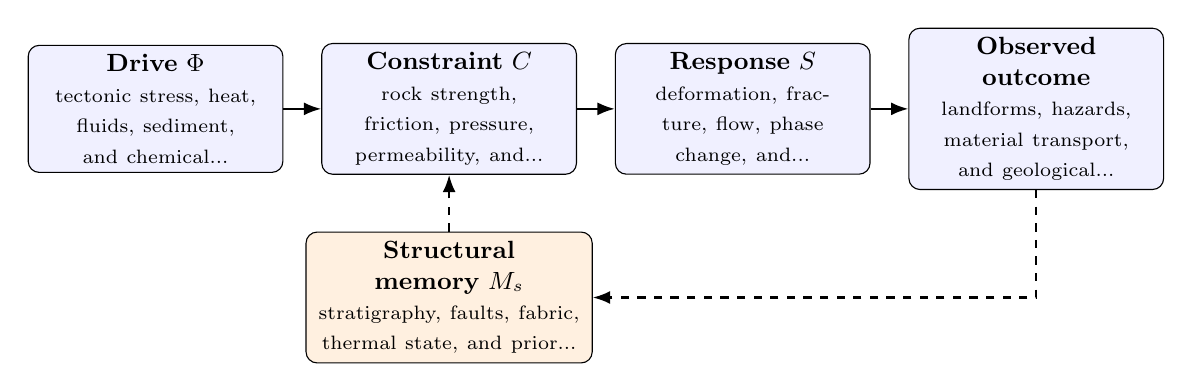
\begin{tikzpicture}[
    node distance=0.48cm,
    every node/.style={font=\small},
    box/.style={draw, rounded corners, align=center, minimum height=1.45cm, text width=3.0cm, fill=blue!6},
    memory/.style={draw, rounded corners, align=center, minimum height=1.25cm, text width=3.4cm, fill=orange!12},
    flow/.style={-{Latex[length=2.2mm]}, thick},
    feedback/.style={-{Latex[length=2.2mm]}, thick, dashed}
]
\node[box] (drive) {\textbf{Drive $\Phi$}\\\scriptsize tectonic stress, heat, fluids, sediment, and chemical...};
\node[box, right=of drive] (constraint) {\textbf{Constraint $C$}\\\scriptsize rock strength, friction, pressure, permeability, and...};
\node[box, right=of constraint] (response) {\textbf{Response $S$}\\\scriptsize deformation, fracture, flow, phase change, and...};
\node[box, right=of response] (outcome) {\textbf{Observed outcome}\\\scriptsize landforms, hazards, material transport, and geological...};
\node[memory, below=0.72cm of constraint] (memory) {\textbf{Structural memory $M_s$}\\\scriptsize stratigraphy, faults, fabric, thermal state, and prior...};
\draw[flow] (drive) -- (constraint);
\draw[flow] (constraint) -- (response);
\draw[flow] (response) -- (outcome);
\draw[feedback] (outcome.south) |- (memory.east);
\draw[feedback] (memory.north) -- (constraint.south);
\end{tikzpicture}
\caption{Paper D-03 observable CDFD/AFL architecture for Geology. Solid arrows give the proposed forward chain; dashed arrows make history-dependent feedback explicit.}
\label{fig:d03-architecture}
\end{figure}

\subsection{Minimal Coupled Model}

A paper-level model must separate throughput, constraint accumulation, response,
and history. One deliberately minimal form is
\begin{align}
Y(t) &= \frac{\Phi(t)S(t)}{\epsilon + C(t)}, \\
\frac{dC}{dt} &= \alpha \Phi(t) - \beta S(t)C(t) + \gamma \mathcal{L}C(t), \\
\frac{dM_s}{dt} &= \eta C(t) - \mu M_s(t), \\
\Psi_s(t) &= \frac{\widehat{\Phi}(t)}{\epsilon+\widehat{C}(t)}\,
             \widehat{S}(t)\,[1+\omega\widehat{M_s}(t)] .
\end{align}
Here $Y$ is the measured output, $\epsilon>0$ prevents a singular denominator,
$\mathcal{L}$ is a spatial or network coupling operator, and hats denote
explicitly normalized variables. The sign and magnitude of $\omega$ must be
estimated: memory can preserve useful organization or amplify damage. No fixed
threshold is universal before the variables, normalization, and observation
scale are declared.

For this paper, the hypothesized causal sequence is specific. A change in
tectonic stress, heat, fluids, sediment, and chemical gradients arrives faster than deformation, fracture, flow, phase change, and chemical alteration can compensate.
This raises or redistributes rock strength, friction, pressure, permeability, and geometry. If the load persists,
the retained state encoded by stratigraphy, faults, fabric, thermal state, and prior deformation changes the next response, so a later event of equal
magnitude can produce a different trajectory in landforms, hazards, material transport, and geological transition. The
scientific task is to estimate that sequence against the best ordinary model of
the domain, not merely to redescribe the outcome after it occurs.

\subsection{Cross-Scale Universality Without Mechanistic Erasure}

For the domain applications family, the universal comparison is a disciplined translation test across systems with very different material mechanisms. A valid mapping preserves the baseline science of the domain, declares the scale of every variable, and earns its place through a discriminating prediction rather than resemblance alone. \cite{Holling1973,Turing1952,Shannon1948,BakTangWiesenfeld1987}
The CDFD programme is cumulative: Part I supplies the flow--constraint
foundation \cite{MujjabiPartI2026}; Part II asks when maintained throughput
supports persistent organized states \cite{MujjabiPartII2026}; Part III
develops adaptive limitation and biological memory \cite{MujjabiPartIII2026};
and Part IV \cite{MujjabiPartIV2026} tests how much of that architecture
survives translation. The CDFD Runtime \cite{CDFDRuntime2026} supplies a
reproducible numerical stress surface, but it does not substitute for the
domain evidence named here.

The required scale declaration for this paper is seconds to billions of years; grains to planets. At short
scales, the key question is whether the incoming drive is transmitted,
buffered, or diverted. At intermediate scales, response changes effective
capacity and network exposure. At long scales, retained structure can alter the
state space itself. A result is genuinely cross-scale only when the aggregation
rule is stated and the same conclusion is not an artifact of averaging.

\subsection{Evidence Ladder and Discriminating Tests}

\begin{table}[htbp]
\centering
\small
\caption{Evidence ladder for Paper D-03. Each rung can fail independently.}
\begin{tabularx}{\textwidth}{|p{0.17\textwidth}|X|X|}
\hline
\textbf{Test} & \textbf{Design} & \textbf{Discriminating result} \\
\hline
Proxy audit & Measure field mapping, geodesy, seismology, petrology, geochemistry, and stratigraphic records and preregister how each record maps to $\Phi$, $C$, $S$, $M_s$, and $Y$. & The mapping fails if proxies are non-identifiable, circular, or change meaning across cases. \\
\hline
Load ramp & Apply or observe a stress or fluid-pressure perturbation across inherited structures while estimating the dominant constraint and response time. & A threshold claim requires a reproducible nonlinear change and uncertainty bounds, not a visually chosen breakpoint. \\
\hline
Recovery and memory & Match present load across units with different histories, then compare recovery paths. & The memory claim requires history-dependent divergence after current conditions are controlled. \\
\hline
Model comparison & Compare the baseline domain model with and without the CDFD/AFL state variables using held-out data. & The paper's stated falsifier is: explicit memory and topology do not improve geological interpretation or prediction. \\
\hline
\end{tabularx}
\end{table}

The strongest practical design combines a prospective perturbation with a
recovery window. The load-ramp phase estimates where constraint begins to rise
faster than output. The recovery phase estimates $\beta$ and $\mu$, separating
fast relaxation from persistent memory. A topology or coupling intervention
then asks whether rerouting changes the cascade as predicted. Null results are
informative because they identify domains in which the universal notation adds
no measurable value.

\subsection{Research Programme and Boundary Conditions}

The immediate research programme has four steps. First, construct a documented
dataset from field mapping, geodesy, seismology, petrology, geochemistry, and stratigraphic records and retain raw units before normalization.
Second, fit a baseline domain model and report its calibration and out-of-sample
error. Third, add the smallest identifiable CDFD/AFL state extension and test
whether it improves prediction of landforms, hazards, material transport, and geological transition. Fourth, repeat the
analysis across the declared scale range and publish negative cases as part of
the universality audit.

Three boundaries are non-negotiable. Correlation between flow and failure does
not identify a constraint mechanism. A fitted memory term does not prove that
the stored state has the same material meaning in another domain. Finally, a
runtime cascade is evidence about the implementation, not evidence that the
real system follows it. The paper becomes stronger when it can say precisely
where the translation stops.


% END PART IV MAJOR UNIVERSAL UPGRADE

\section{Conclusion}

Geological systems are AFL flux--constraint systems operating at planetary scales. Earthquakes,
volcanic eruptions, plate tectonics, and induced seismicity all emerge from the universal AFL
equation with domain-appropriate $(\Phi, C)$ interpretation. The Gutenberg-Richter law, seismic
cycle periodicity, and eruption style are AFL predictions derivable from constraint heterogeneity
and the ratio $\Psi_s^* = J/C$.

\bibliographystyle{plain}
\bibliography{universal_afl_references}

\end{document}